\level{1}{Descrizione generale dei prodotti}
    Riportiamo di seguito una descrizione generale dei prodotti. Per una descrizione più dettagliata delle funzionalità dei prodotti, si rimanda al documento \insdoc{Analisi dei Requisiti v6.00}.

    \level{2}{Norris}
        \insglo{Norris} è un \insglo{framework} per \insglo{Node.js} che permette di raccogliere dati provenienti da sorgenti arbitrarie e visualizzarli come grafici in modo semplice e veloce. In particolare mette a disposizione dei suoi utenti due interfacce:
        \begin{itemize}
            \item le \insglo{API} interne (lato \insglo{server});
            \item le \insglo{API} esterne (lato \insglo{client}).
        \end{itemize}
        
        \level{3}{API interne}
        Tramite le \insglo{API} interne, uno sviluppatore può creare quattro tipologie di grafici: \insglo{bar chart}, \insglo{line chart}, \insglo{map chart} e \insglo{table}. Per ogni grafico può configurare le relative impostazioni e può impostare il metodo di aggiornamento dei dati del grafico stesso. L'aggiornamento dei grafici può essere di tre tipologie, a seconda del tipo di grafico:
        \begin{itemize}
            \item \insglo{in place}, supportato da tutti i tipi di chart;
            \item \insglo{stream}, supportato da \insglo{bar chart}, \insglo{line chart} e \insglo{table};
            \item \insglo{movie}, supportato da \insglo{map chart}.
        \end{itemize}
        
        Lo sviluppatore può, inoltre, scegliere di incapsulare alcuni grafici all'interno di una o più pagine web. Le \insglo{API} interne permettono infatti di aggiungere i grafici creati ad una o più pagine web, le quali verranno create in automatico da \insglo{Norris}. Lo sviluppatore, oltre a poter scegliere quali grafici inserire in queste pagine, può configurare le impostazioni di ciascuna di esse. Tra le impostazioni principali ci sono la scelta del titolo e del template della pagina.\\
        Infine, se lo sviluppatore non vuole rendere pubblici i propri grafici, può definire una funzione login, una funzione isLogged e una funzione di logout. Queste verranno eseguite ogni qualvolta venga richiesto di accedere alle informazioni di un grafico.
       
        \level{3}{API esterne}
            Tramite le \insglo{API} esterne, un utente lato \insglo{client} può effettuare l'autenticazione ad un'istanza di \insglo{Norris} esistente e richiedere al \insglo{server} le informazioni inerenti ai grafici presenti in quell'istanza. In particolare l'utente \insglo{client} può richiedere la lista dei grafici presenti nell'istanza, nonché le informazioni di ogni singolo grafico della lista. Le informazioni verranno fornite in formato \insglo{JSON}.

    \level{2}{Chuck}
        \insglo{Chuck}, acronimo di Chart Universal Creator Kit, è una libreria \insglo{JavaScript} lato \insglo{client} che permette di incapsulare un grafico (creato tramite le \insglo{API} interne di \insglo{Norris}) all'interno di una pagina web diversa da quelle create di default da \insglo{Norris}. In particolare lo sviluppatore lato \insglo{client} deve autenticarsi ad un'istanza di \insglo{Norris}, richiedere un grafico e scegliere il tag HTML in cui inserire il grafico. È possibile, inoltre, modificare alcune impostazioni relative al grafico.
    
    \level{2}{Applicazione Android}
        L'applicazione \insglo{Android} permette di visualizzare i grafici di un'istanza di \insglo{Norris} da uno smartphone \insglo{Android}. Essa permette di scegliere l'istanza di \insglo{Norris} alla quale connettersi tramite autenticazione. Una volta autenticato, l'utente può visualizzare la lista di grafici esistenti e i grafici stessi.
    \level{2}{Dashboard APS}
        La \insglo{dashboard} rappresenta un caso d'uso di \projectname{}. In particolare, essa è un'applicazione web utile alla visualizzazione di informazioni riguardanti le linee degli autobus dell'\insglo{APS} di Padova, con aggiornamento real-time.\\
        Attraverso l'uso di una mappa, l'utente finale potrà vedere gli spostamenti, in tempo reale, dei mezzi di trasporto della rete urbana.\\
    
        
\level{1}{Descrizione delle interazioni che i prodotti hanno tra di loro}
    \level{2}{Norris - Chuck}
        \insglo{Norris} e \insglo{Chuck} interagiscono tramite le \insglo{API} esterne, le quali fungono da interfaccia tra \insglo{server} e \insglo{client}. In particolare si possono avere 3 tipologie di interazione:
        \begin{itemize}
            \item autenticazione: precede l'invio di informazioni inerenti un grafico. \insglo{Chuck} manda a \insglo{Norris} l'indirizzo dell'istanza a cui si vuole connettere, assieme ad username e password. \insglo{Norris} controlla se i dati inviati sono corretti e, in caso affermativo, esegue l'autenticazione. Riportiamo di seguito un diagramma esplicativo:
        	\begin{figure}[H]\centering
        		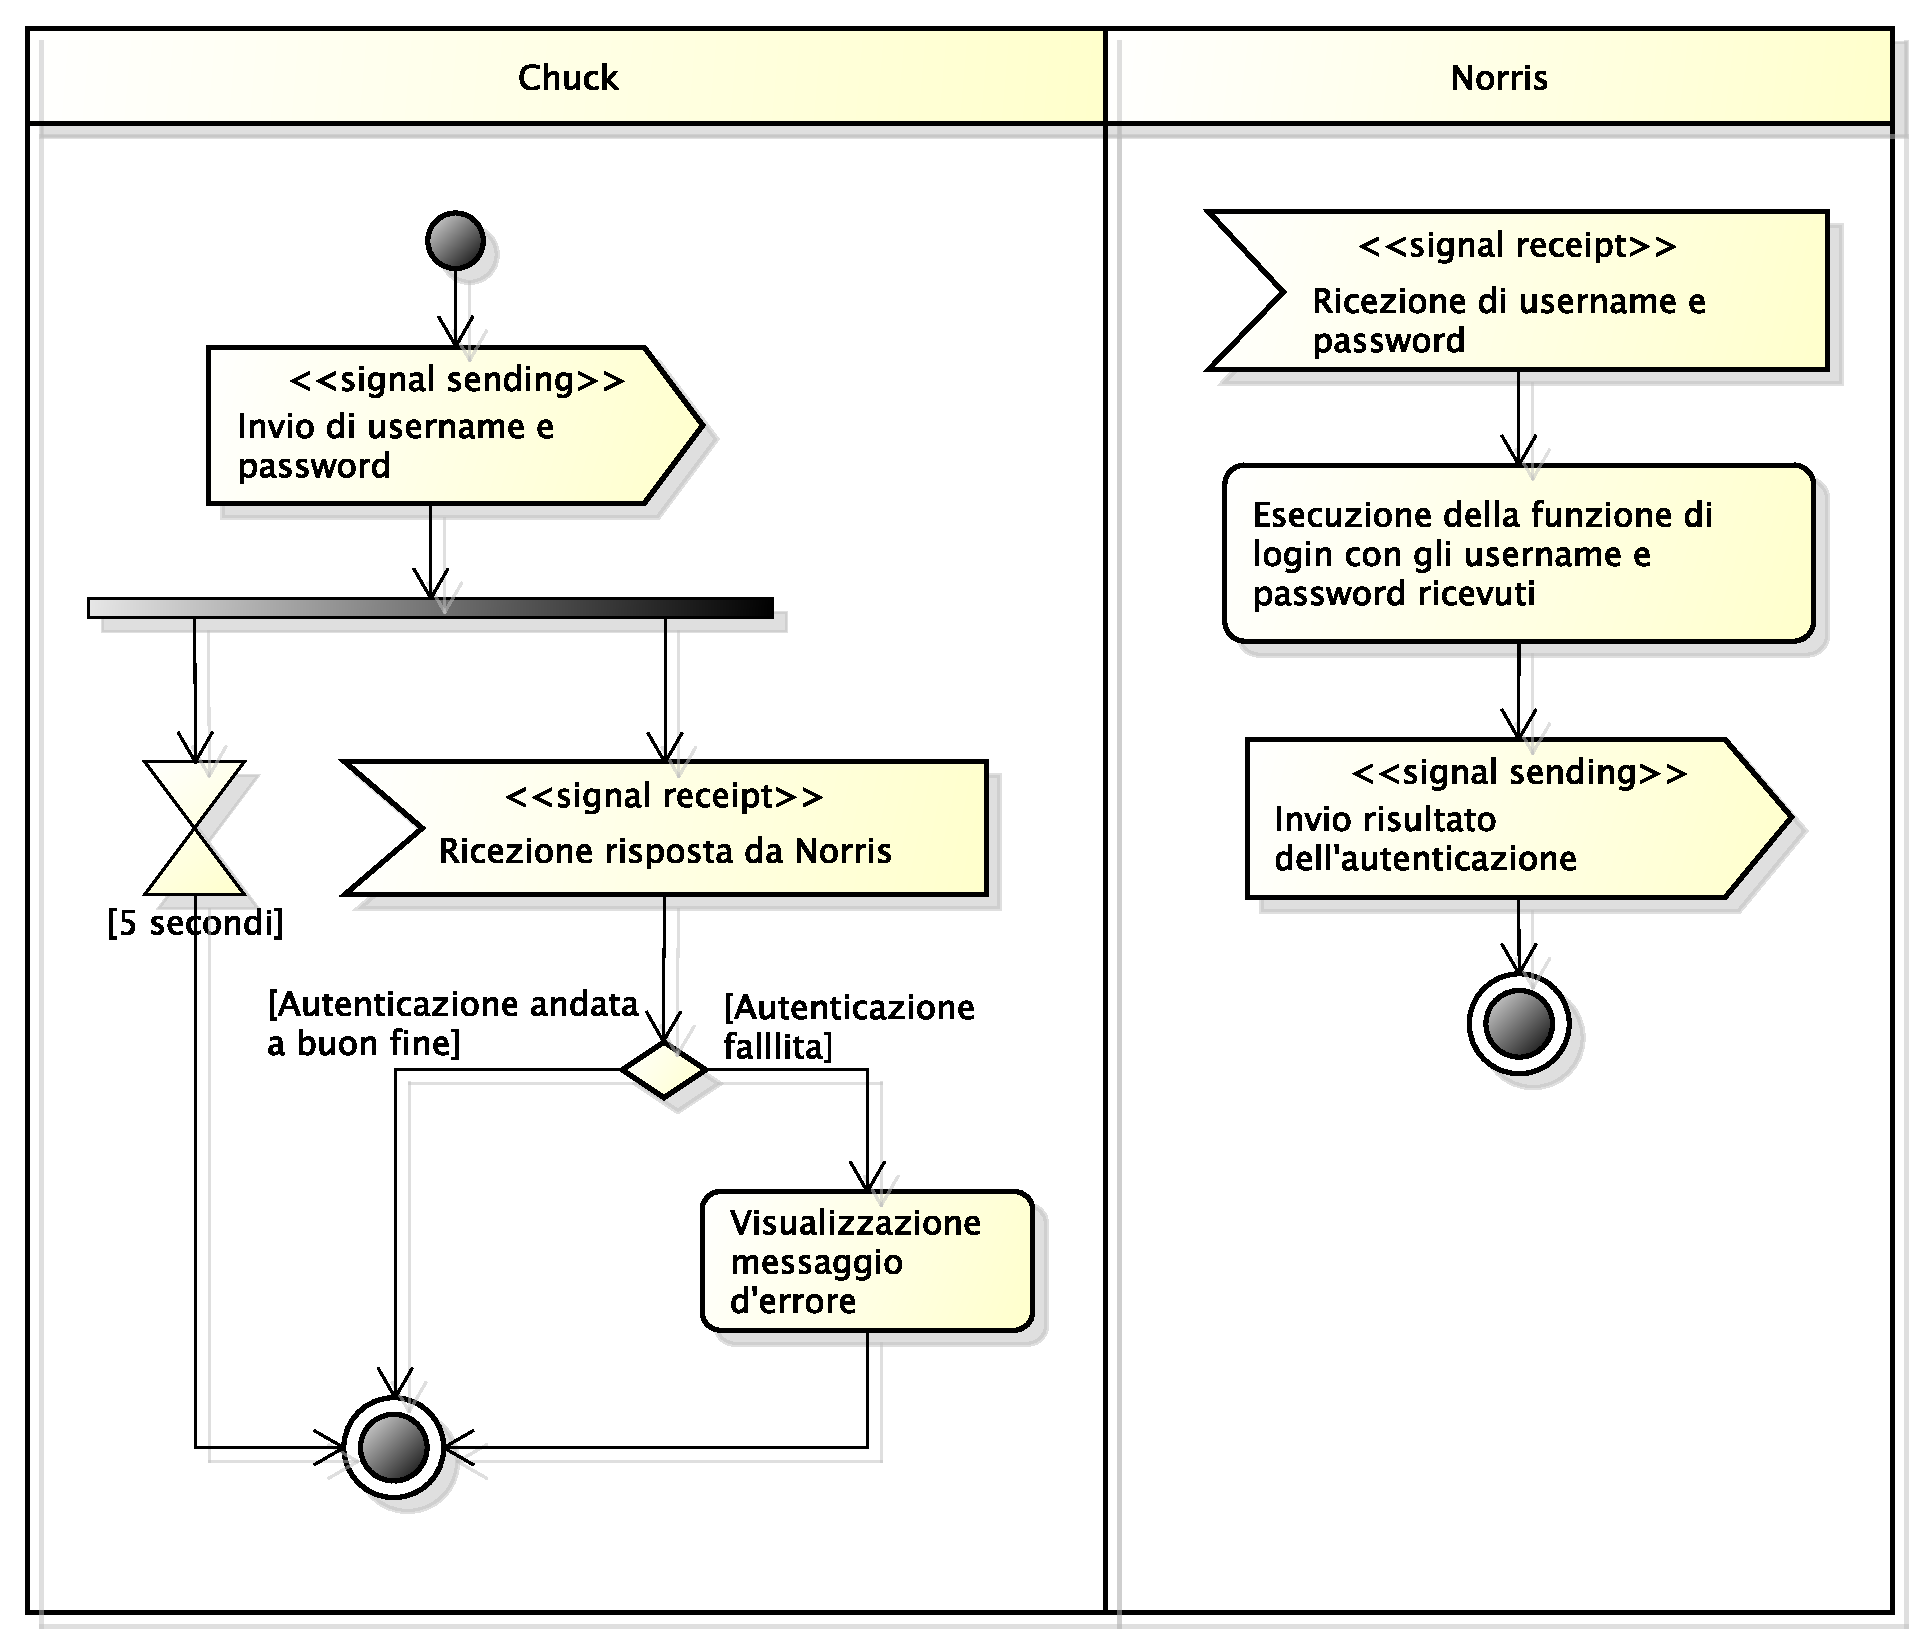
\includegraphics[width=\textwidth]{SpecificaTecnica/Pics/Chuck/Autenticazione.pdf}
        		\caption{Diagramma di attività dell'autenticazione}
    		\end{figure}
	
            \item richiesta inserimento grafico: \insglo{Chuck} manda a \insglo{Norris} una richiesta di informazioni inerenti al grafico che si vuole inserire nella pagina web. \insglo{Norris} controlla se il \insglo{client} è autenticato. In caso negativo, \insglo{Norris} manda una richiesta di autenticazione al \insglo{client}. In caso affermativo, invece, \insglo{Norris} manda le informazioni relative al grafico richiesto aprendo una comunicazione tramite \insglo{websocket}. Il canale rimane aperto fintanto che il \insglo{client} rimane connesso. Riportiamo di seguito un diagramma esplicativo:
            \begin{figure}[H]\centering
        	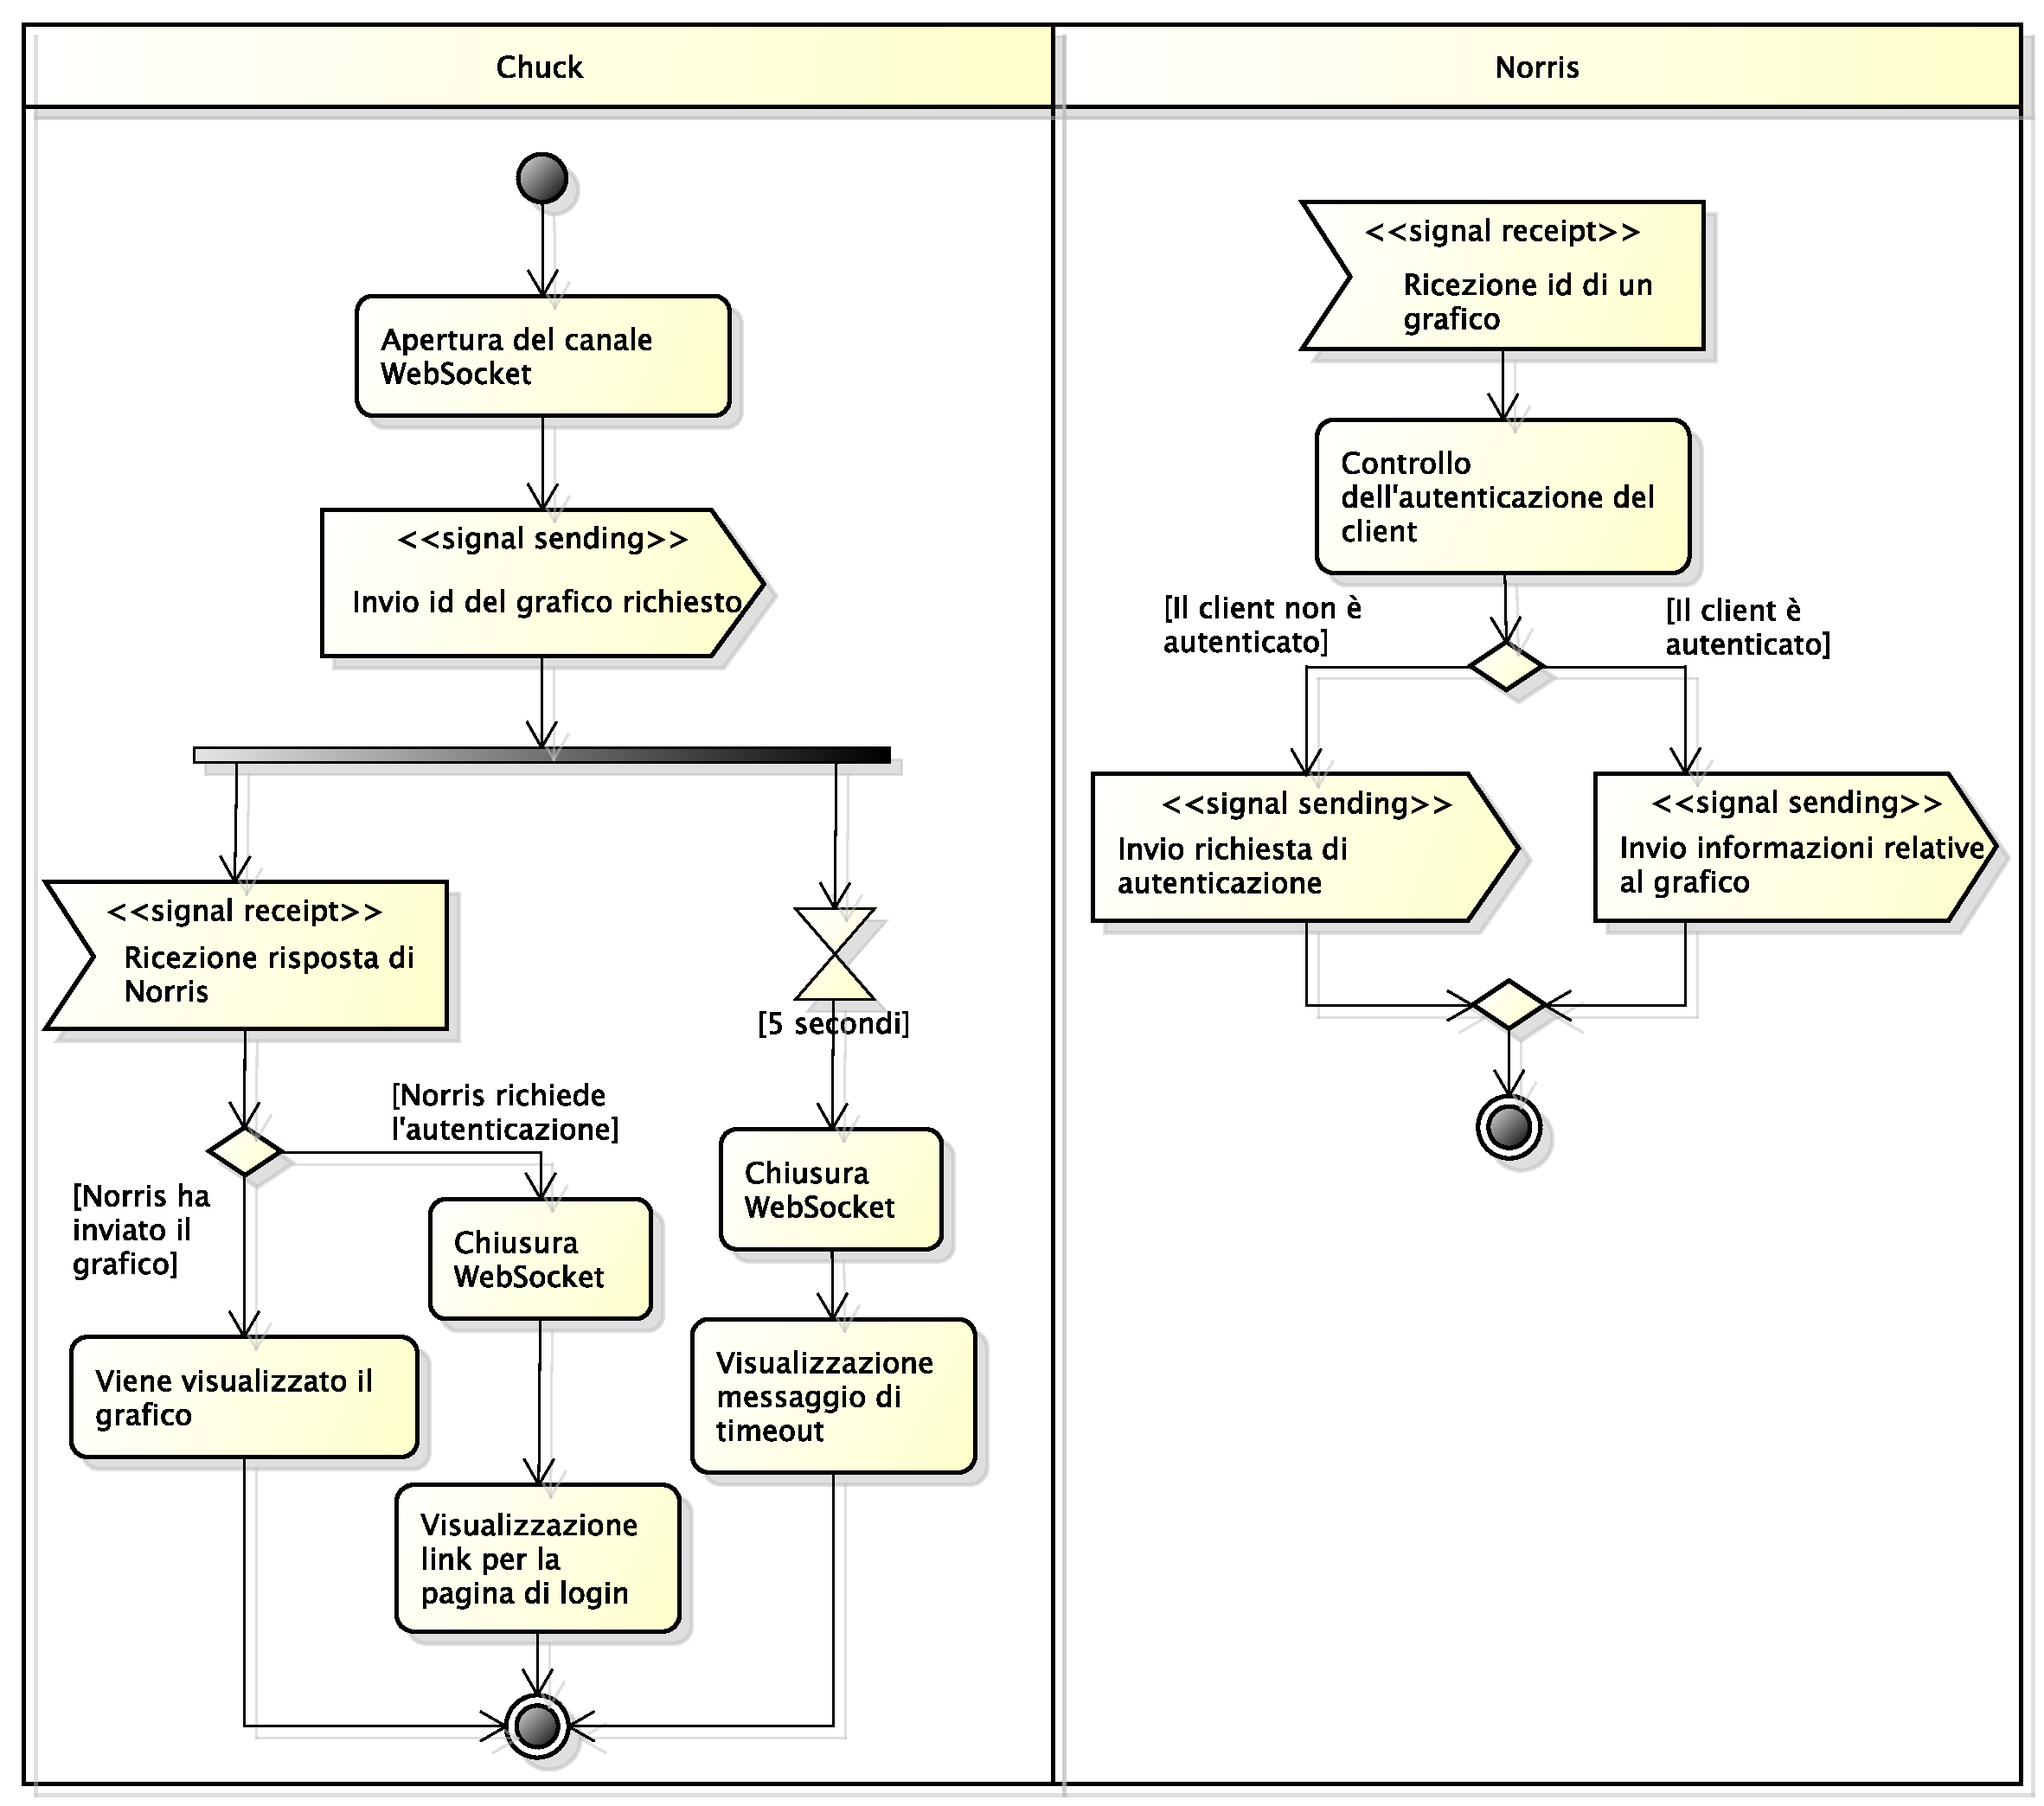
\includegraphics[width=\textwidth]{SpecificaTecnica/Pics/Chuck/RichiestaGrafico.pdf}
        	\caption{Diagramma di attività della richiesta di inserimento di un grafico}
    		\end{figure}
            \item aggiornamenti del grafico: quando un grafico viene aggiornato lato \insglo{server}, \insglo{Norris} si preoccupa di mandare l'aggiornamento ai \insglo{client} che hanno quel grafico. La comunicazione dell'aggiornamento avviene tramite un canale \insglo{websocket} appositamente creato al momento della richiesta di inserimento del grafico nella pagina web. Riportiamo di seguito un diagramma esplicativo:
            \begin{figure}[H]\centering
        	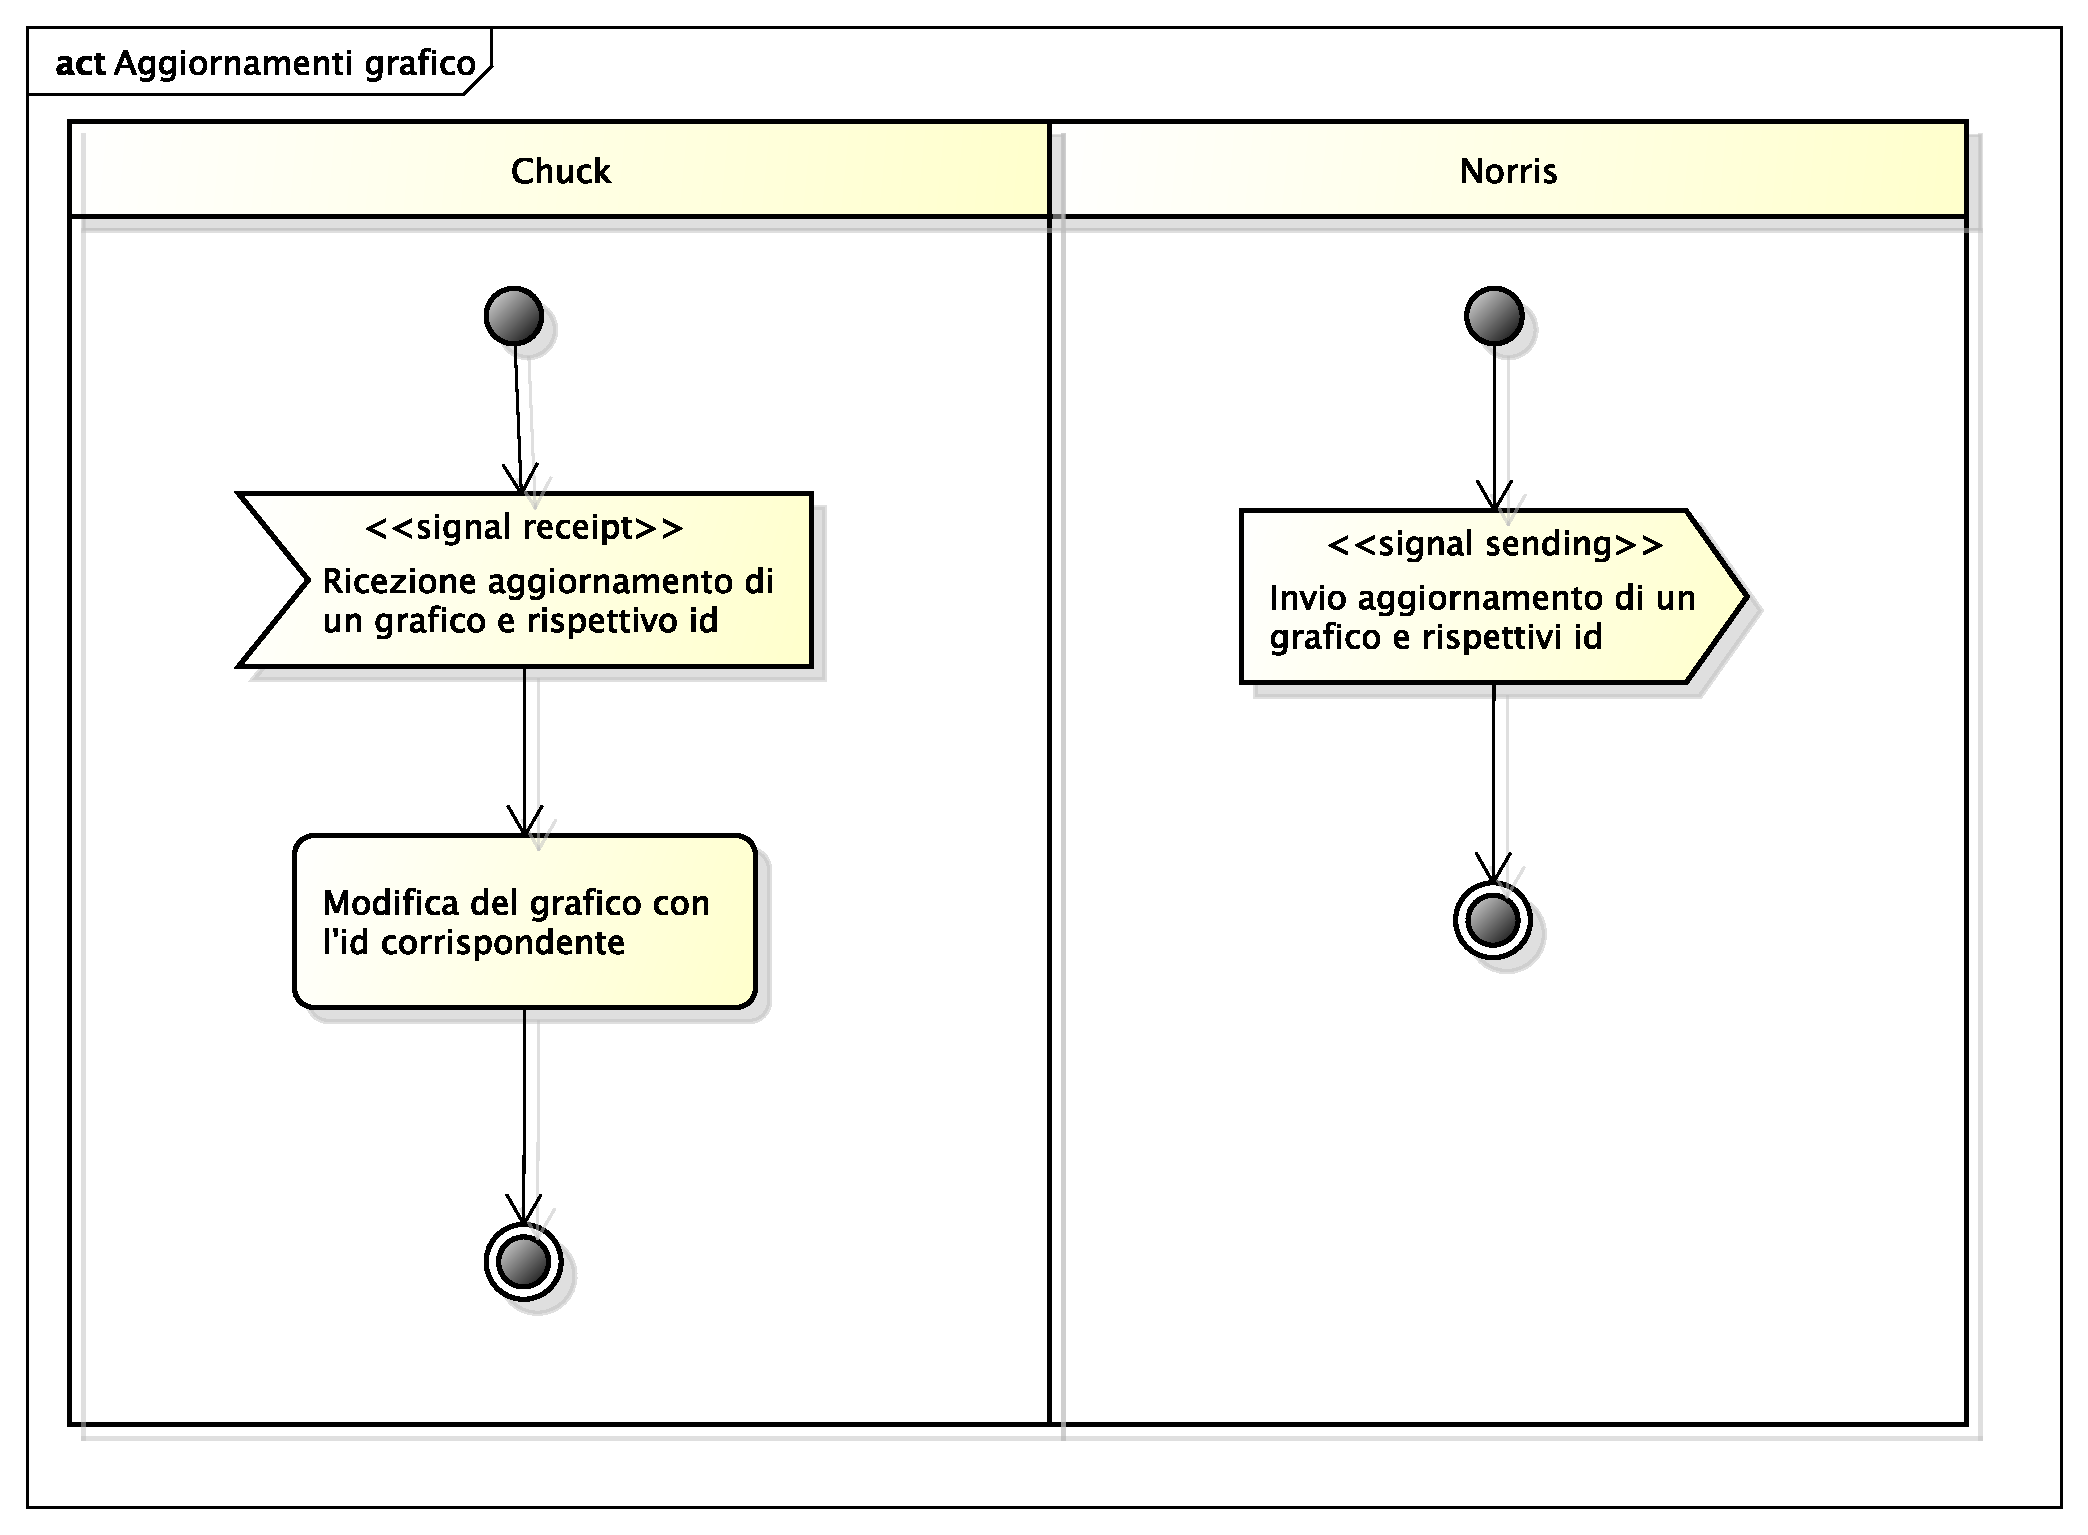
\includegraphics[width=\textwidth]{SpecificaTecnica/Pics/Chuck/AggiornamentiGrafico.pdf}
        	\caption{Diagramma di attività dell'aggiornamento di un grafico}
    		\end{figure}
        \end{itemize}
    
    \level{2}{Norris - Applicazione Android}
        \insglo{Norris} e l'applicazione \insglo{Android} interagiscono tramite le \insglo{API} esterne, le quali fungono da interfaccia tra \insglo{server} e \insglo{client}. In particolare si possono avere 4 tipologie di interazione:
        \begin{itemize}
            \item Autenticazione: precede l'invio di informazioni inerenti un grafico. L'applicazione \insglo{Android} manda a \insglo{Norris} l'indirizzo dell'istanza a cui si vuole connettere, assieme ad username e password. \insglo{Norris} controlla se i dati inviati sono corretti e, in caso affermativo, esegue l'autenticazione. Se l'autenticazione non va a buon fine, l'applicazione \insglo{Android} mostra un messaggio d'errore. Riportiamo di seguito un diagramma esplicativo:
        	\begin{figure}[H]\centering
        		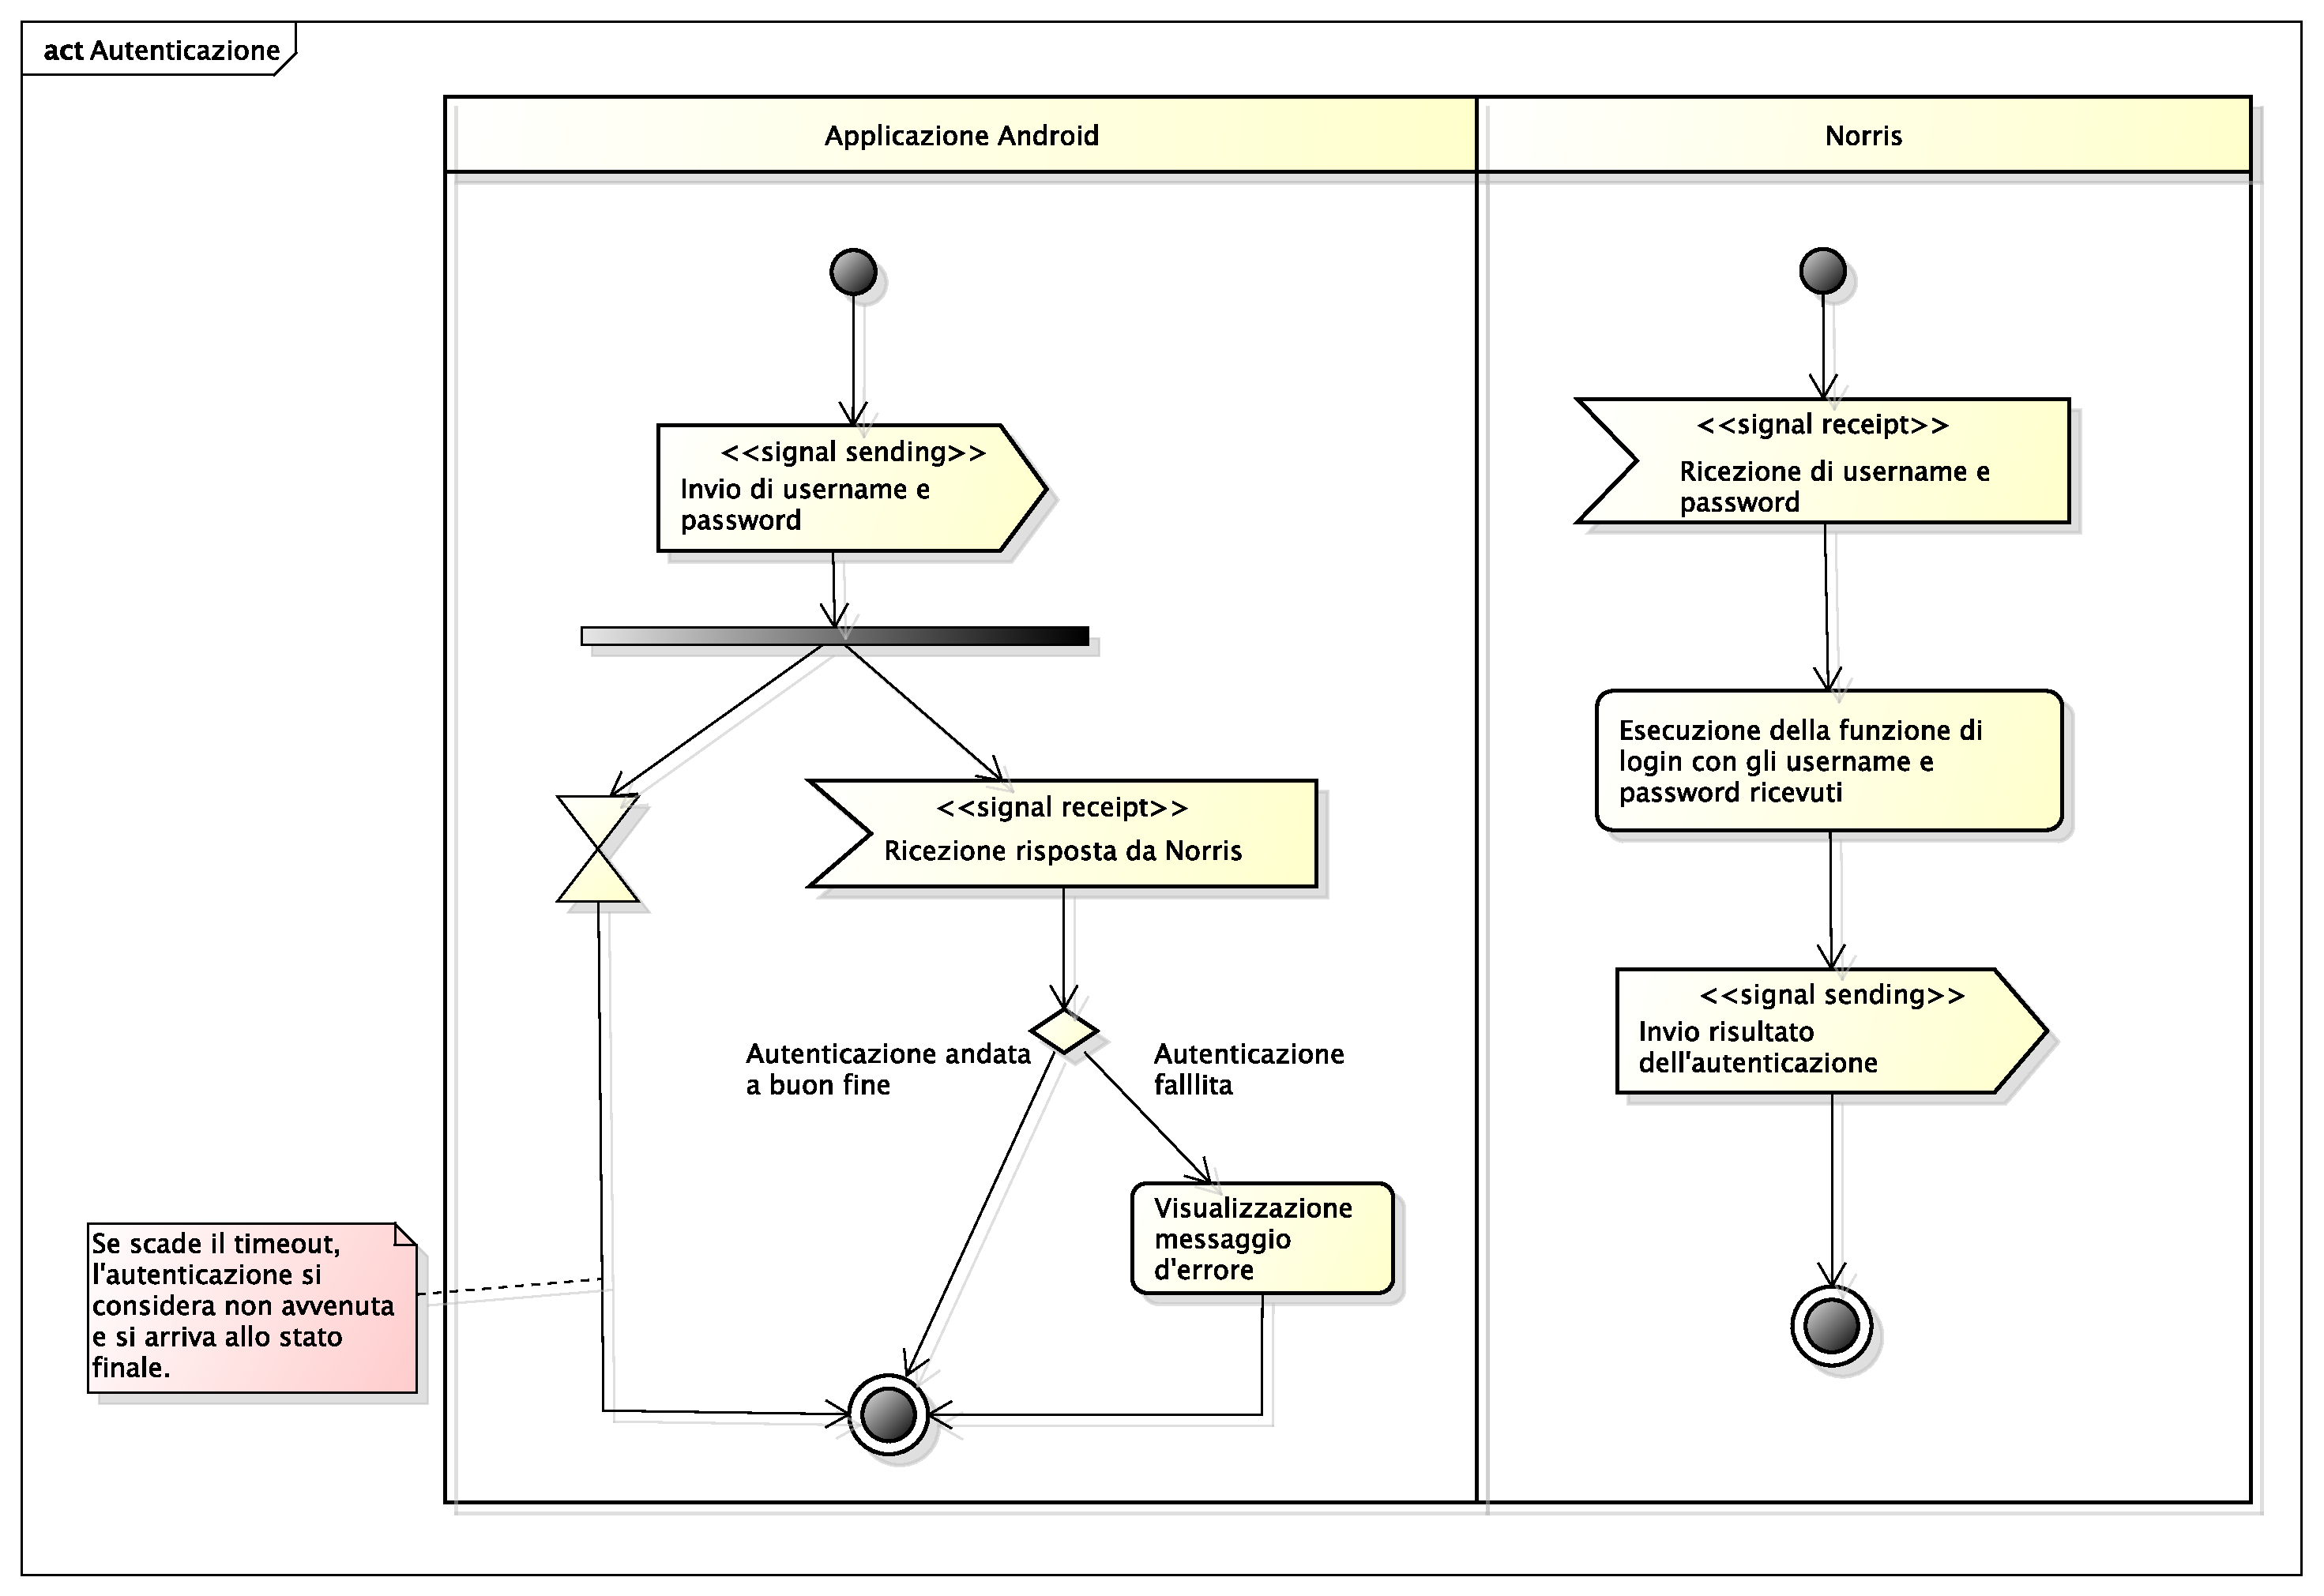
\includegraphics[width=\textwidth]{SpecificaTecnica/Pics/Applicazione/Autenticazione.pdf}
        		\caption{Diagramma di attività dell'autenticazione}
    		\end{figure}
            \item Richiesta informazioni della lista di grafici: l'applicazione \insglo{Android} manda a \insglo{Norris} una richiesta di informazioni inerenti alla lista di grafici presenti nell'istanza di \insglo{Norris} alla quale ci si è autenticati. \insglo{Norris} controlla se l'utente è autenticato e, in caso affermativo, manda le informazioni relative alla lista di grafici richiesta tramite una richiesta \insglo{HTTP}. Riportiamo di seguito un diagramma esplicativo:
            \begin{figure}[H]\centering
        	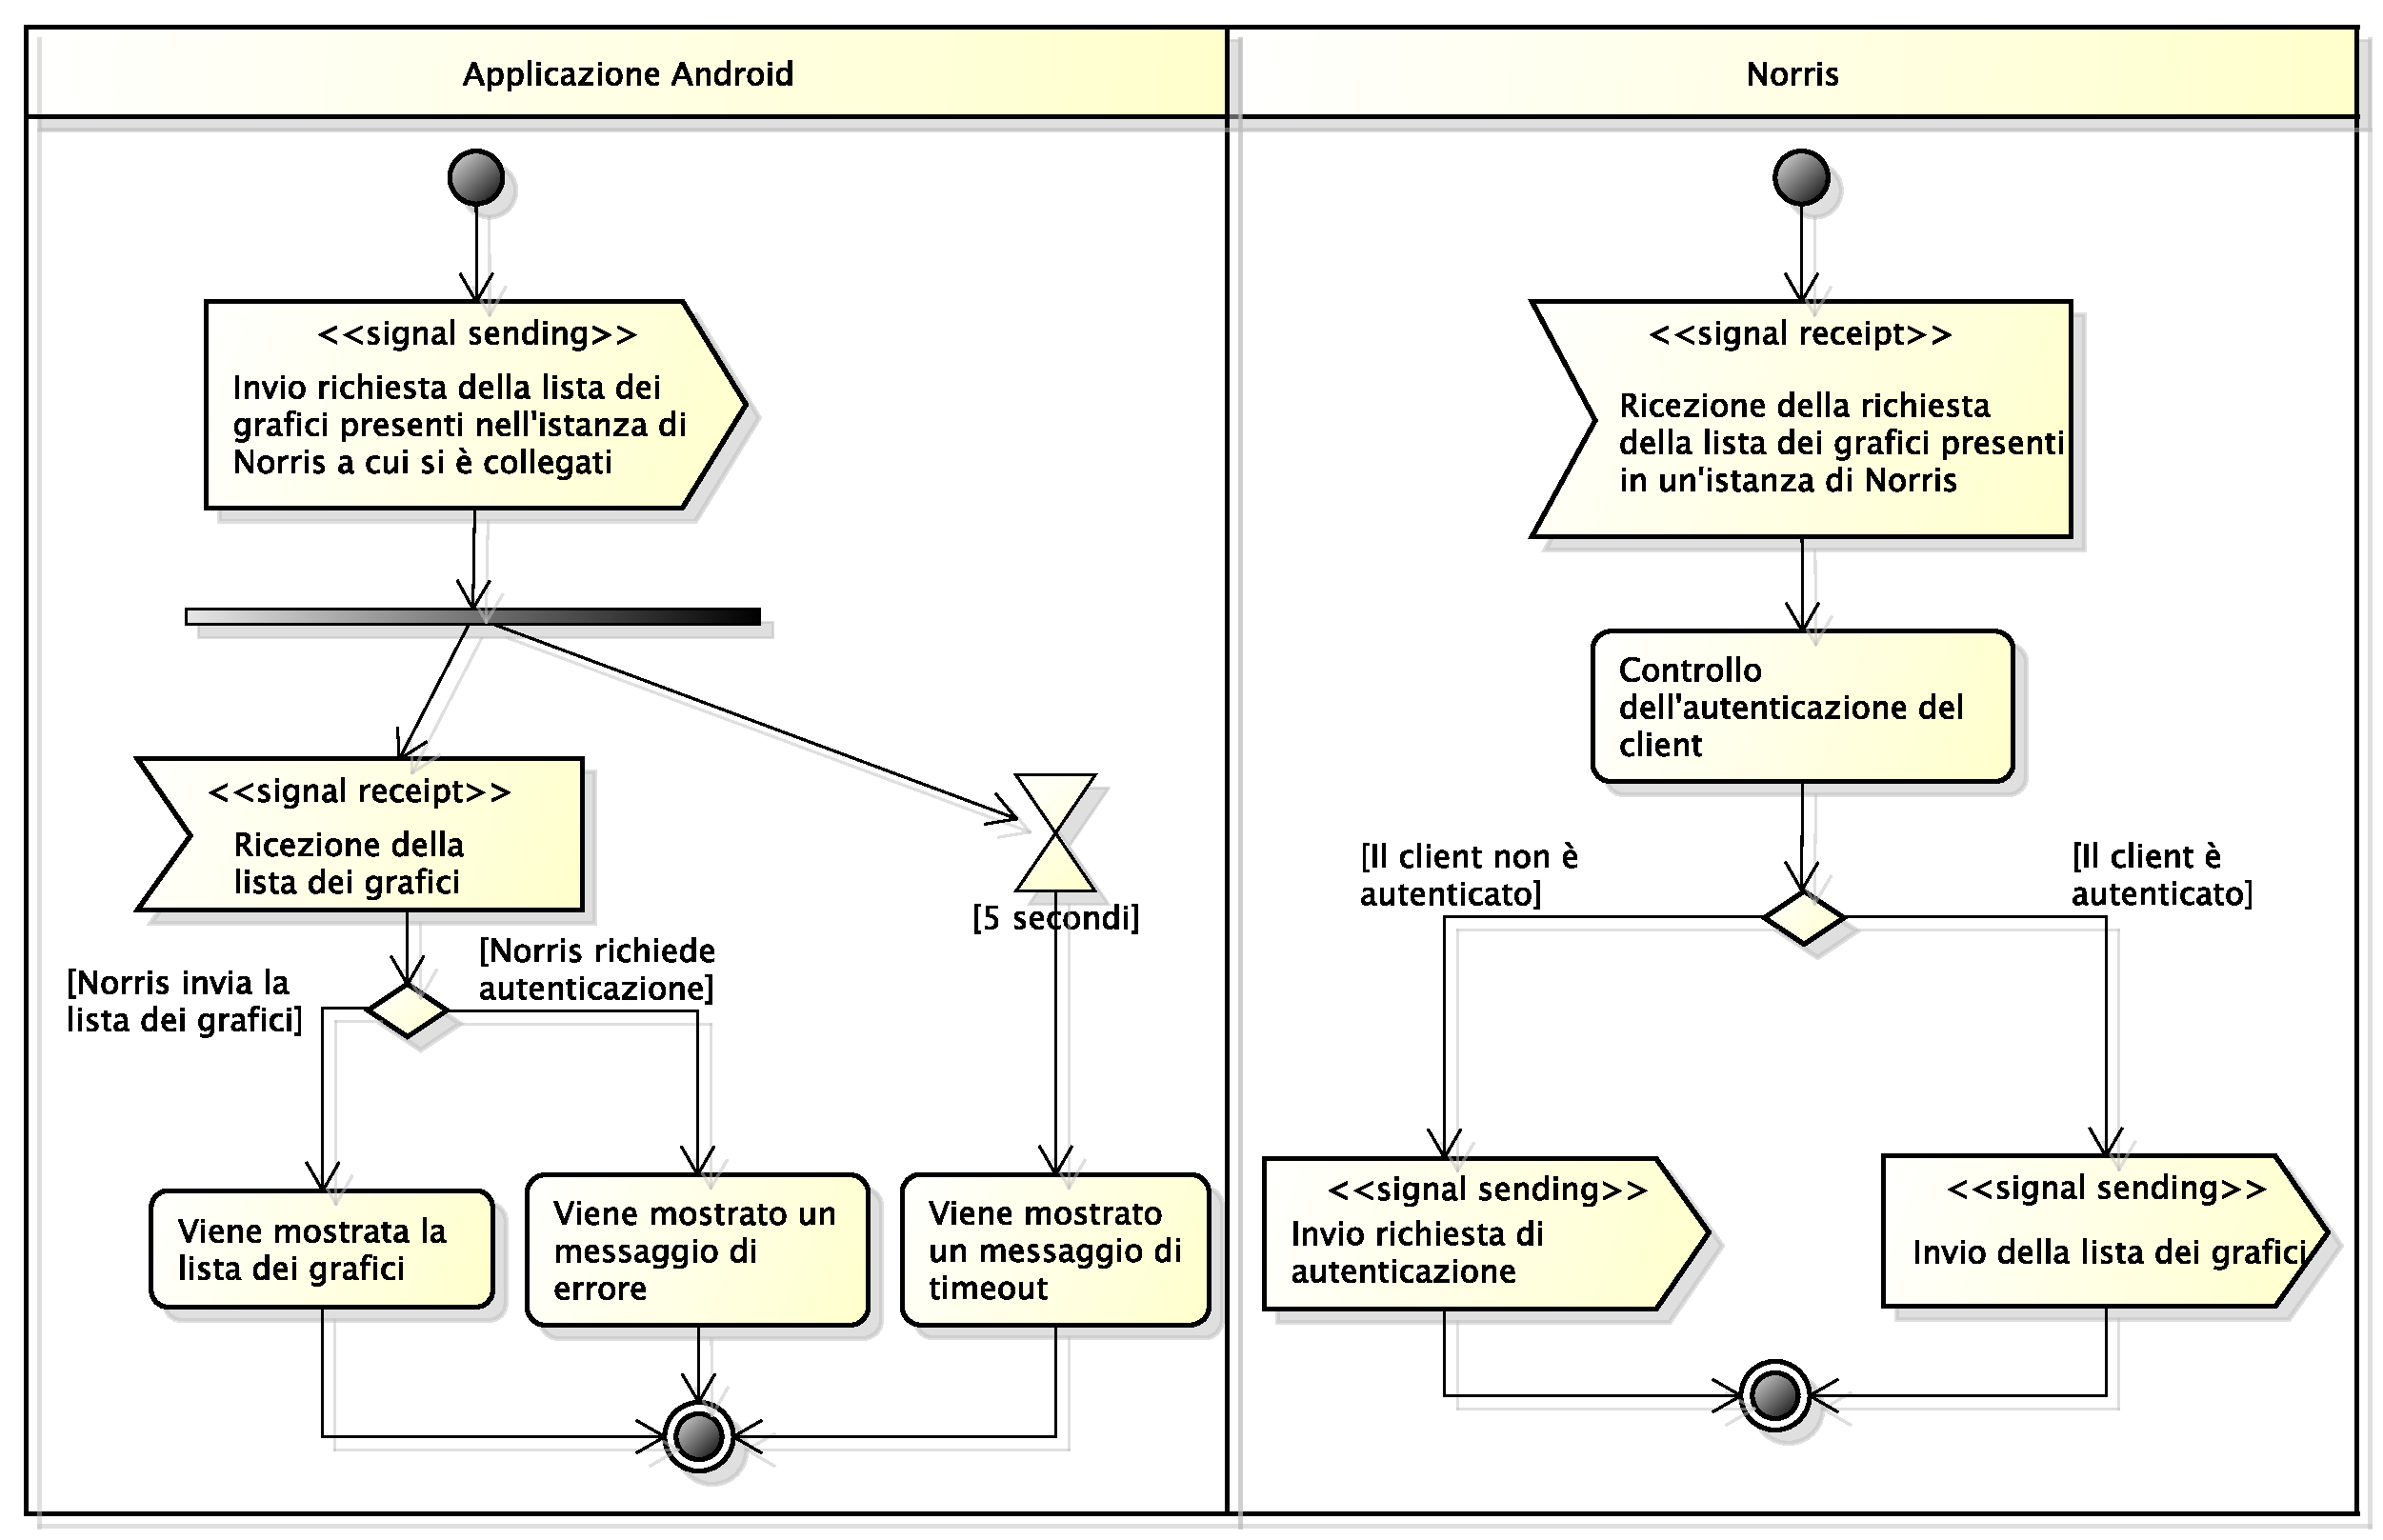
\includegraphics[width=\textwidth]{SpecificaTecnica/Pics/Applicazione/RichiestaLista.pdf}
        	\caption{Diagramma di attività della richiesta delle informazioni di una lista di grafici}
    		\end{figure}
            \item Richiesta informazioni di un grafico: l'applicazione \insglo{Android} manda a \insglo{Norris} una richiesta di informazioni inerenti al grafico che si vuole visualizzare nell'applicazione. \insglo{Norris} controlla se il \insglo{client} è autenticato e, in caso affermativo, manda le informazioni relative al grafico richiesto aprendo una comunicazione tramite \insglo{websocket}. Il canale viene chiuso quando il grafico o l'applicazione sono in background. Riportiamo di seguito un diagramma esplicativo:
            \begin{figure}[H]\centering
        	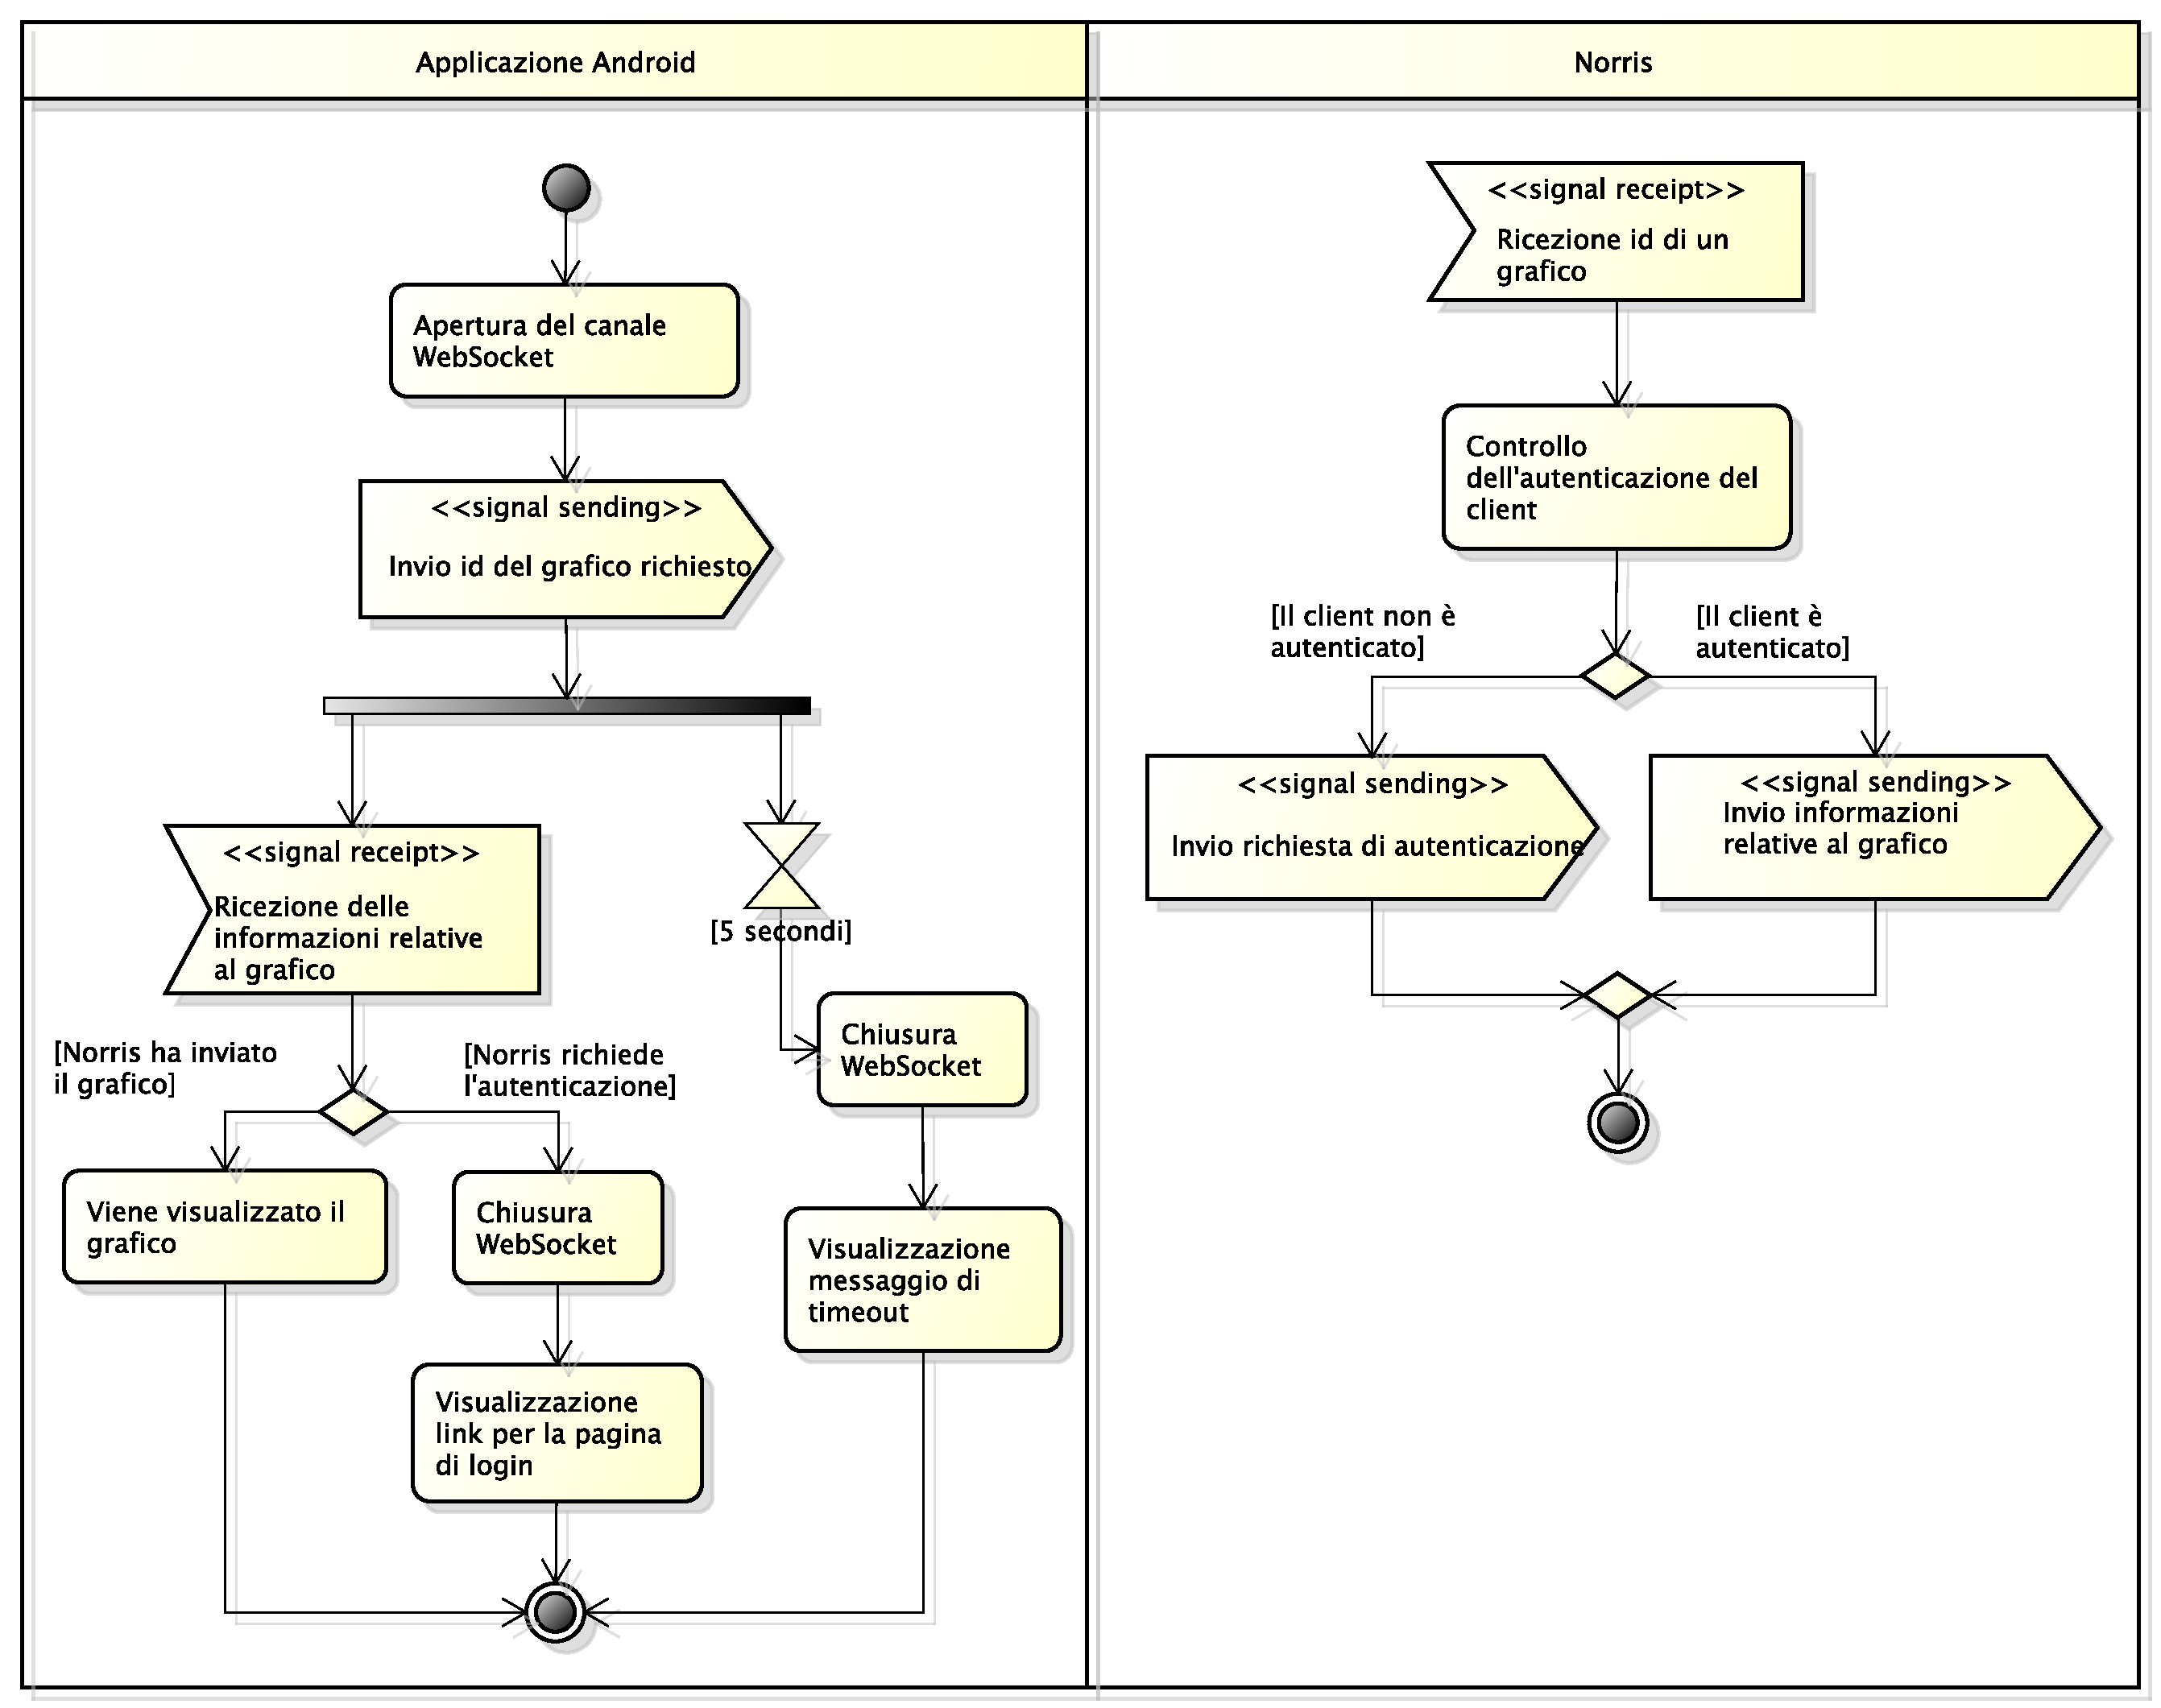
\includegraphics[width=\textwidth]{SpecificaTecnica/Pics/Applicazione/RichiestaGrafico.pdf}
        	\caption{Diagramma di attività della richiesta delle informazioni di un grafico}
    		\end{figure}
            \item Aggiornamenti del grafico: quando un grafico viene aggiornato lato \insglo{server}, \insglo{Norris} si preoccupa di mandare l'aggiornamento ai \insglo{client} che hanno quel grafico. La comunicazione dell'aggiornamento avviene tramite un canale \insglo{websocket} appositamente creato al momento dell'invio dell'aggiornamento. Il canale viene chiuso quando il grafico o l'applicazione sono in background. Gli aggiornamenti avranno luogo solo quando il grafico è attivo. Se il grafico è in background, gli aggiornamenti vengono ignorati. Riportiamo di seguito un diagramma esplicativo:
            \begin{figure}[H]\centering
        	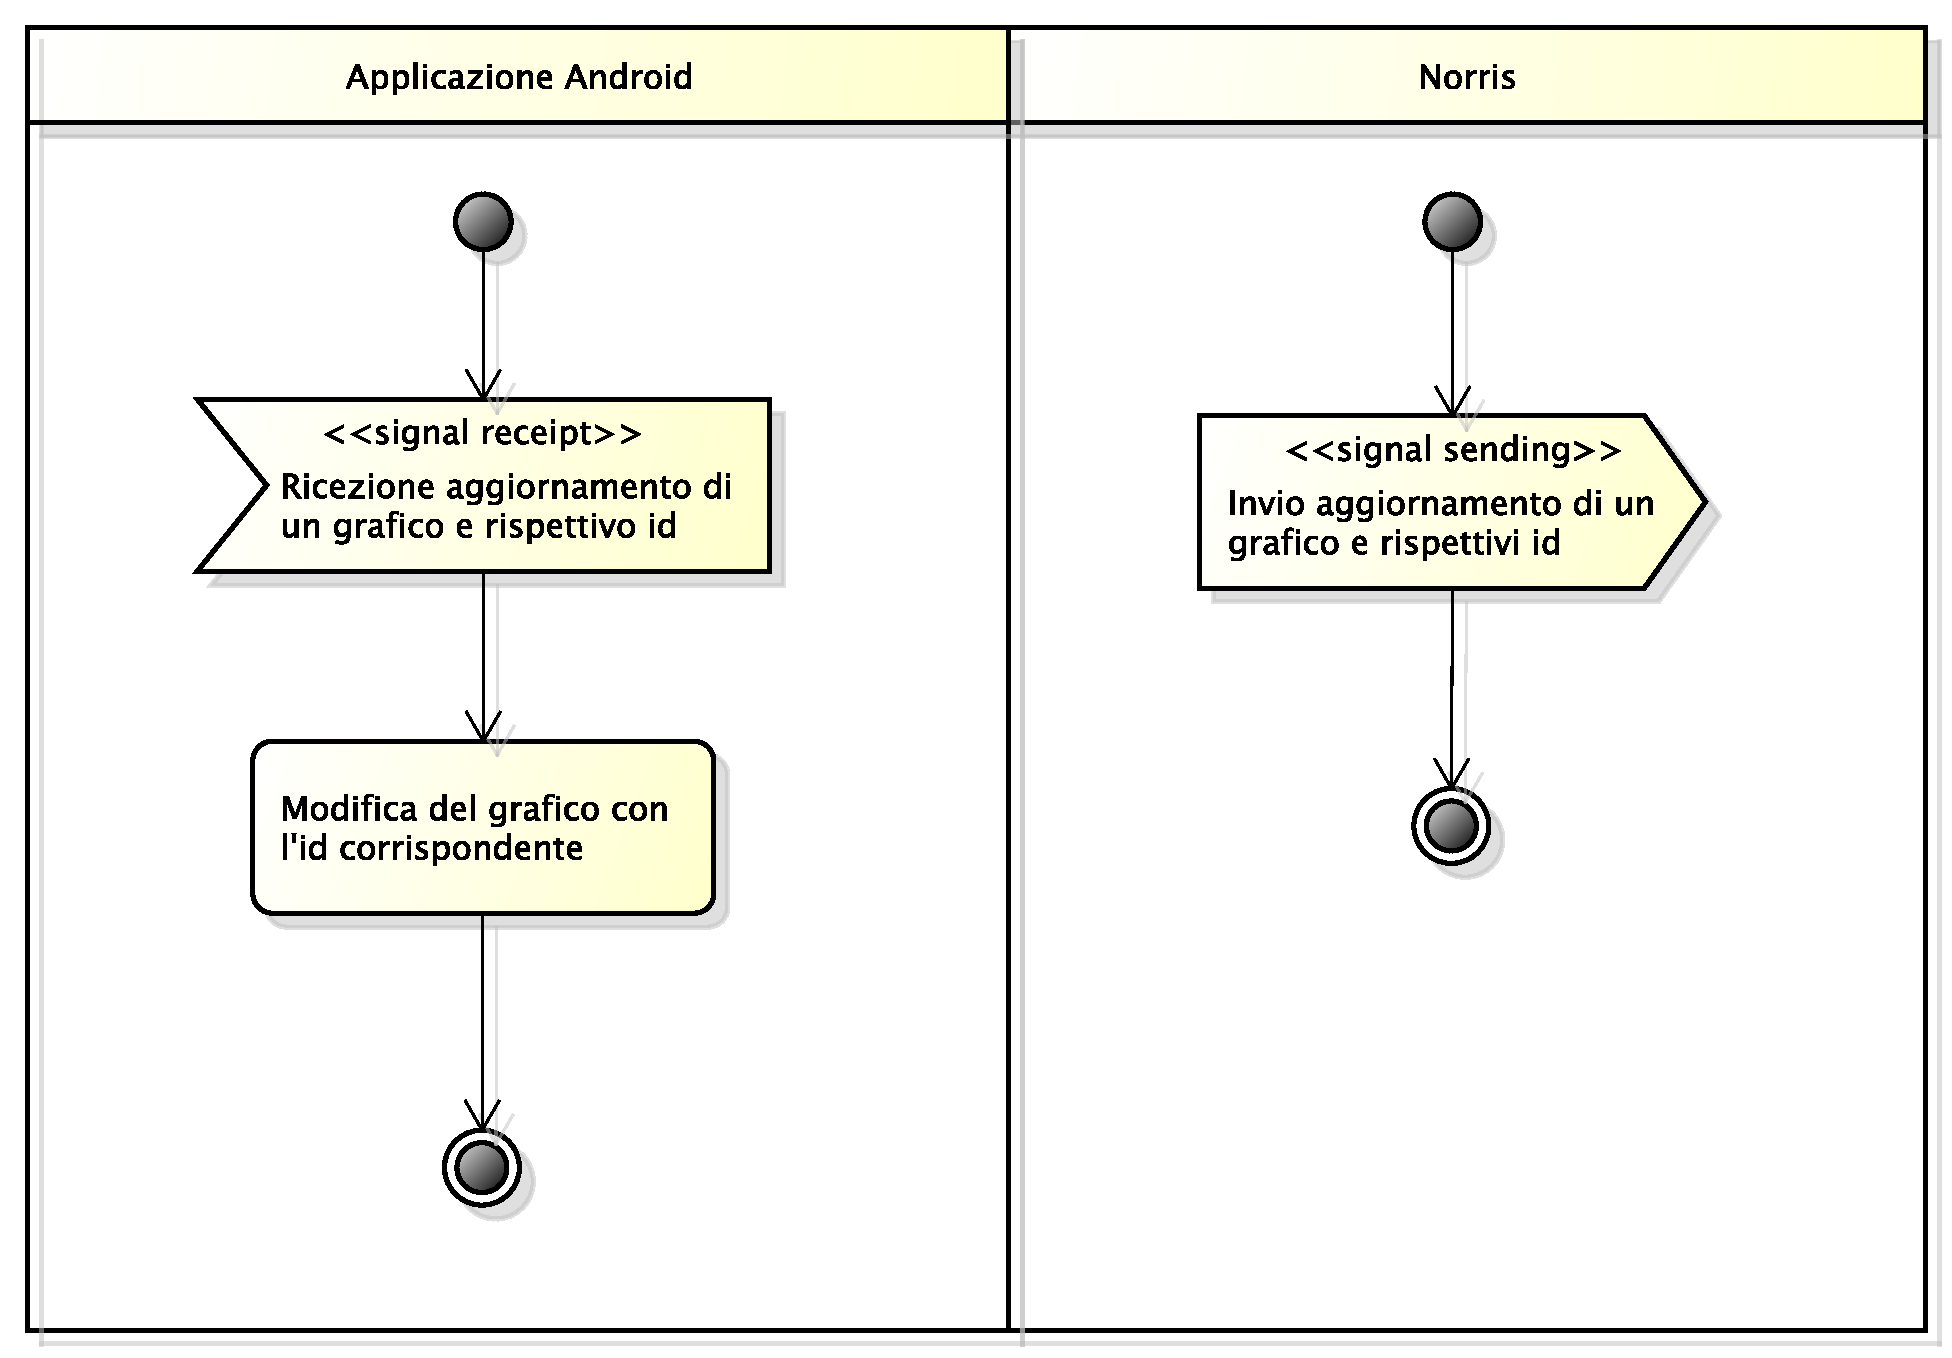
\includegraphics[width=\textwidth]{SpecificaTecnica/Pics/Applicazione/AggiornamentiGrafico.pdf}
        	\caption{Diagramma di attività dell'aggiornamento di un grafico}
    		\end{figure}
        \end{itemize}
